\documentclass[11pt,a4paper]{article}
\usepackage{microtype}
\usepackage{lecght}
\usepackage{times}\let\Bbbk\relax\let\vec\relax
%\usepackage{txfonts}\let\Bbbk\relax
\usepackage{mtpro2}
\usepackage{bm}
\usepackage{helvet}
\usepackage{datetime}
\usepackage{tikz}
\usepackage{enumerate}

\newcommand{\cN}{\mathcal{N}}
\newcommand{\be}{\begin{equation}}
\newcommand{\ee}{\end{equation}}
\newcommand{\ra}{\rightarrow}
\newcommand{\reals}{\mathbb{R}}
\newcommand{\idf}{1\!\!1}
\newcommand{\mL}{\textrm{MoveLeft}}
\newcommand{\mR}{\textrm{MoveRight}}
\newcommand{\eps}{\varepsilon}
\newcommand{\wt}{\marginpar{[*]}}

\setlength{\parindent}{0pt}
\addtolength{\oddsidemargin}{-1in}
\addtolength{\textwidth}{1.75in}
\addtolength{\topmargin}{-0.5in}
\addtolength{\textheight}{2in}

\renewcommand{\arraystretch}{2}

\begin{document}
\ddmmyyyydate
\graphicspath{{/Users/ht/Library/SUlogo/}}

\pagestyle{plain}

\vspace*{-0.7in}
\hfill\resizebox{2.5in}{!}{
\includegraphics{../../info/icts.pdf}}%

\vspace*{-18mm}

{\huge
A Short Course in

\vspace*{1ex}

Reinforcement Learning\\
}

\vspace*{-7mm}

\section{Coursework 1}

\begin{itemize}
\setlength{\itemsep}{0pt}
\item Problems marked with * in the margin are for weeks 2 and 3.
\item Solutions will be posted after week 3.
\end{itemize}

\begin{enumerate}[\bf Q1.]
\item \textbf{($\mathbf{k}$-armed bandit problem)} A slot machine has 3 levers, numbered from 0 to 2, that returns a random reward $R$ with distribution $\cN(a,1)$, where $a=0,1,2$ is the lever number interpreted as an ``action''. Not knowing the underlying distribution of rewards, you ``act'' on the slot machine by pulling its levers many times until you find or ``learn'' the winning lever giving the largest expected reward
\[
Q^* = \max_a Q(a) = \max_a \mathbb{E}[R|a].
\]
\begin{enumerate}[\bf (a)]
\item Write a program that ``pulls'' each lever in succession 1000 times and records the rewards obtained for each. Compare the histograms and means of the rewards obtained.
\item Let $(A_i)_{i=1}^n$ be a sequence of actions (i.e., lever number pulled) and $(R_i)_{i=1}^n$ the corresponding sequence of rewards. Write a function that takes as input these two sequences and returns the estimated value function
\[
Q_n(a) =\frac{\sum_{i=1}^n R_i \idf_{A_i=a}}{\sum_{i=1}^n  \idf_{A_i=a}}
\]
for each action $a=0,1,2$. Here $\idf_{A_i=a}$ is the indicator function equal to 1 if $A_i=a$ and 0 otherwise. Your function should have no nested loops and its output should be an array of 3 elements. Set $Q_n(a)=-\textrm{inf}$ for any action not present or seen in a trajectory.

\item An $\eps$-greedy policy for learning the winning lever proceeds as follows:
\begin{enumerate}[1-$\!\!$]
\item Initialise action list with $[A_1]$ and reward list with the corresponding reward $[R_1]$
\item Calculate $Q_1(a)$ using the function of Part (b)
\item With probability $\eps$: Select next action $A_2$ randomly. With complementary probability $1-\eps$: Select next action as
\[
A_2 = \arg\max_a Q_1(a)
\]
\item Add $A_2$ and its corresponding reward $R_2$ in their respective list
\item Repeat Steps 2-4 with current lists $N$ times.	
\end{enumerate}
Implement this algorithm. In the end, show the accumulated reward averaged over time as a function of time (i.e., iteration number) from $n=1$ to $n=N=1000$. Repeat for $\eps=0, 0.1, 0.3$, showing the results on the same plot. Re-run your code until you get a curve close to $2$, the max expected reward. Explain your results.

\item The value function $Q(a)$ can be estimated more efficiently using the following stochastic approximation:
\[
Q_n (a) = (1-\alpha_n) Q_{n-1}(a) + \alpha_n R_n
\]
for the realised action $A_n=a$ at time $n$ (with corresponding reward $R_n$) and
\[
Q_n(a') = Q_{n-1}(a')
\]
for all other actions $a'\neq a$. Here $\alpha_n=1/n$ is the annealing sequence. Implement this iteration and plot as in Part (c) the accumulated reward averaged over time for $\eps=0, 0.1, 0.3$. Use $Q_0(a)=0$ for the initial value in the iteration. Re-run your code until you get a curve close to $2$, the max expected reward. Explain your results.
\end{enumerate}

\item \textbf{(Linear model: Markov reward process)} We consider the simple linear model with 7 states, discussed in class. The reward is a function $r(s)$ of the current state $S_t =s\in \{0,2,\ldots, 6\}$, taken to be $r(0)=1$, $r(6)=10$, and $0$ otherwise. Thus $R_{t+1}$ is deterministic given $S_t=s$, and is equal to $1$ when leaving state $0$ and $10$ when leaving state $6$.
\begin{center}
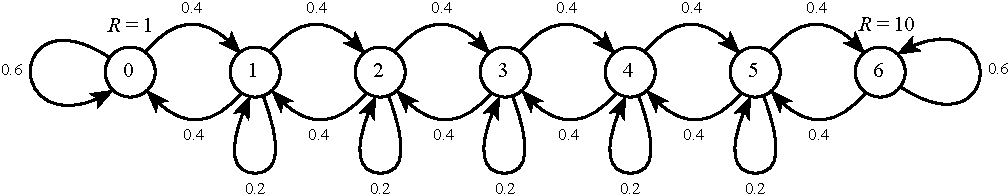
\includegraphics[width=0.8\textwidth]{marsroverexample1-crop.pdf}
\end{center}
\begin{enumerate}[\bf (a)]
\item For the transition probabilities $p(s'|s)$ shown above, calculate the value function $v(s)$ by directly solving the linear Bellman equation. Show the result as a plot for the values for $s=0,1,\ldots,6$. Repeat the calculation for $\gamma=0,0.1,0.2,\ldots, 0.9$ and show the results on the same plot.
\item Calculate \wt $v(s)$ by solving the linear Bellman equation iteratively. Show the results as in Part (a).
\item Write a program that generates one trajectory of the Markov reward process from time $t=1$ to $t=N$ and the return accumulated over that time. Pay attention to the extremal states $0$ and $6$. 
\item Estimate $v(2)$ for $\gamma=0.5$ using many simulated trajectories. Try different sample sizes (numbers of trajectories) and final times to make sure your results converge. Compare with the result of Part (a).
\end{enumerate}

\item \textbf{(Linear model: Markov decision process)} We modify the model of Q2 to make it a decision process by including two types of deterministic actions for each state: 
\begin{itemize}
\item $\mR$ action ($a=1$): Move from state $S_{t}=i$ to $S_{t+1}=i+1$, unless $S_t=6$ in which case stay there so $S_{t+1}=6$:
\begin{center}
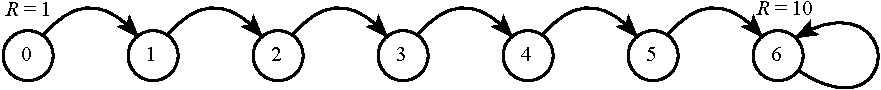
\includegraphics[width=0.7\textwidth]{moveright1-crop.pdf}
\end{center}
\item $\mL$ action ($a=0$): Move from state $S_t=i$ to $S_{t+1}=i-1$ unless $S_t=0$ in which case stay there so $S_{t+1}=0$:
\begin{center}
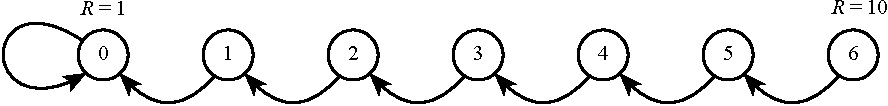
\includegraphics[width=0.7\textwidth]{moveleft1-crop.pdf}
\end{center}
\end{itemize}

\begin{enumerate}[\bf (a)]
\item Write down the transition probabilities $p(s'|s,a)$ for $a=0$ and $a=1$ as two $7\times 7$ matrices.

\item Calculate the value function $v_\pi(s)$ for the full $\mR$ policy, $\pi(s)=1$ for all $s$, by solving the linear Bellman equation directly. Show the result in a plot as in Q2(a). Repeat for the full $\mL$ policy, $\pi(s)=0$ for all $s$, and then for the random $\frac{1}{2}\mL+\frac{1}{2}\mR$ policy. Compare and explain your results.

\item Write \wt down the Bellman optimality equation for $v_*(s)$ and simplify it knowing that there are only two actions to compare and only one $s'$ for a given $s$ when $s$ is not an extremal state  (0 or 6). What is the simplified equation for the extremal states? You should end up with a max over two expressions for $a=0,1$.

\item Use \wt your simplified Bellman optimality equation in an iterative way to find the optimal value function $v_*(s)$ for $\gamma=0.5$ and the corresponding optimal (deterministic) policy $\pi_*(s)$, represented as $0,1$. The optimal policy is obtained iteratively as the solution of the max at each iteration. Use synchronous updating in the iteration by copying $v_k$ into a temporary vector. Show on the same plot $v_*(s)$ and the $v(s)$ obtained before for the fixed $\mL$ and $\mR$ policies. Explain your results.

\item (Optional) Repeat \wt Part (d) using in-place or asynchronous updating without the temporary copy of $v_k$.

\item Suppose \wt you add a third action, called Stay, such that $S_{t+1}=S_t$ for all states. Explain why adding this action does not change the optimal value function and optimal policy. Would the optimal solution change if moves from state $3$ to state $6$ were added?
\end{enumerate}

\item \textbf{(Linear model: Temporal difference)} \wt
\begin{enumerate}[\bf (a)]
\item Implement the TD(0) algorithm for finding the value function $v_\pi(s)$ associated with the random $\frac{1}{2}\mL+\frac{1}{2}\mR$ policy	 for the linear model. Use $\gamma=0.5$, $\alpha=0.1$, 1000 episodes, and $N=1000$ time steps per episode. Only show the final estimates, comparing the estimated $v_\pi$ with the result found in Q3 on the same plot. %[See Sutton \& Barto, p.~98]
\item Implement the Sarsa algorithm for finding $q_*$ and $\pi_*$ for the linear model. Use $\gamma=0.5$, $\alpha=0.2$, $\eps=0.1$, 1000 episodes, and $N=1000$ time steps. Only show the final estimates. %[See Sutton \& Barto, p.~106]
\item Implement the Q-learning algorithm for finding $q_*$ and $\pi_*$ as in Part (b). %[See Sutton \& Barto, p.~107]
\item Explain the difference between Sarsa and Q-learning. 
\end{enumerate}

\item \textbf{(Gridworld)} \wt Use the Q-learning algorithm to find the optimal value function and policy of the gridworld model found in Sutton \& Barto, p.~60. Compare with the optimal solution obtained for $\gamma=0.9$ (with $\eps=0.1$ and $\alpha=0.2$) shown on p.~65.
\end{enumerate}

\section{Coding tips}

\begin{itemize}
\item Don't define functions to answer a question, e.g., def Q1(bla, bla, bla).
\item Never write a function that returns a plot.
\item Don't define functions if you don't intend to use them more than 3 times.
\item Don't re-use bits of code if you can use a loop instead.
\item Clean your code: no unnecessary spaces, variables, containers, while True loops, etc. 
\item Code briefly but clearly. Don't over-write code and avoid being pythonic.
\item Organise your notebook: use sections, subsections, etc., and put a header with your name.
\end{itemize}

\vfill
Hugo Touchette\hfill Version: \today\ \currenttime

\end{document}